\graphicspath{{"./Chapter 2/Figures/"}}

\chapter{Generation of karst networks}
\label{chap:karsts}
\minitoc

- ...

\section{Introduction}
\label{sec:karst_introduction}
- Definition: complex subterranean systems formed primarily in soluble rocks like limestone, dolomite, and gypsum. \\
- Importance: significant for water resources, unique ecosystems, and land use management. \\
- Formation and development \\
** Chemical weathering \\
*** Study the role of rainwater acidity (carbonic acid) in dissolving carbonate minerals. \\
** Underground drainage \\
*** Analyze the development of subterranean drainage systems, including caves, tunnels, and sinkholes. \\
** Speleogenesis \\
*** Examine the process of cave formation, especially at or below the water table. \\
- Key features of karst networks \\
** Caves and caverns \\
*** Document major cave systems and their formation processes. \\
** Sinkholes (dolines) \\
*** Identify areas prone to sinkhole formation and study their causes. \\
** Disappearing streams and springs \\
*** Trace the path of streams that vanish into the ground and re-emerge. \\
** Karst valleys \\
*** Investigate valleys formed by the collapse of underground voids. \\
** Stalactites and stalagmites \\
*** Study the formation of these features within caves. \\
- Hydrology of karst networks \\
** Aquifers \\
*** Assess the productivity and structure of karst aquifers. \\
** Groundwater flow \\
*** Model the rapid and turbulent flow of water through karst systems. \\
** Vulnerability to contamination \\
*** Evaluate the risks and sources of contamination in karst aquifers. \\
- Ecology of karst environments \\
** Unique habitats \\
*** Research cave-dwelling species (troglobites) and their adaptations. \\
** Biodiversity hotspots \\
*** Identify and document biodiversity hotspots in karst regions. \\
- Human interaction with karst networks \\
** Water resources \\
*** Study the dependence of regions on karst aquifers for freshwater. \\
** Tourism \\
*** Assess the impact of tourism on karst landscapes and caves. \\
** Land use challenges \\
*** Develop guidelines for construction and land use planning in karst regions. \\
** Environmental concerns \\
*** Identify and mitigate pollution and land degradation impacts. \\
- Examples of karst regions \\
** The Mammoth Cave System (USA): world's longest cave system. \\
** The Guilin Karst (China): unique limestone peaks and river systems. \\
** The Dinaric Karst (Balkans): extensive cave systems and karst phenomena. \\
- Research and study in karst science \\
** Speleology \\
*** Promote the scientific study of caves and karst features. \\
** Geohydrology \\
*** Conduct studies on water flow in karst systems for resource management. \\
** Geomorphology \\
*** Research the development of karst landforms over geological timescales. \\
- Action steps \\
** Field surveys and mapping \\
*** Conduct detailed field surveys and create maps of karst features. \\
** Hydrological studies \\
*** Implement hydrological modeling and water quality testing. \\
** Ecological research \\
*** Carry out biodiversity assessments and ecological studies in karst habitats. \\
** Human impact analysis \\
*** Study the impact of human activities on karst systems and develop mitigation strategies. \\
** Education and outreach \\
*** Educate local communities and stakeholders about the importance of karst networks and sustainable practices. \\
- Goals \\
** Conservation \\
*** Preserve unique karst ecosystems and landscapes. \\
** Sustainable development \\
*** Ensure that human activities in karst regions are sustainable and minimize environmental impacts. \\
** Scientific advancement \\
*** Promote research and understanding of karst processes and features.

\section{Related works}
\label{sec:karsts_related-works}
- State of the art: \\
** \cite{Paris2021} \\
*** In our case, we do not rely on a graph and path finder, which allows us to compute sections of the karst on the fly (no need to know the whole network to find paths) \\
** \cite{Pytel2015} \\
*** Based on voxels, looks plausible, with a low number of parameters, but take way too long (\~10 to 20 minutes per generation) \\
*** Which makes it unfit for user interaction \\
** \cite{Collon2015,Collon2017} \\
- With some imagination, we can see the shape of trees: \\
** [Prusinkiewicz : ANY] \\
** \cite{Runions2008} \\
- Or miscelleanous networks: \\
** \cite{Galin2010, DiasFernandes2018} \\
- Maybe even look for lychen or ant colonies \\
- ...

\section{Space colonization}
\label{sec:karsts_space-colonization}
- Not really a tree, but... \\
** Some networks are branching \\
** Some have low number of cycles \\
- SC is easy to manipulate for an user \\
- For these reasons, we will consider the use of SC. \\
- Description of the algorithm: \\
** Definition of a root and sinks \\
** Evolution from the root toward closest sinks \\
** Branching [WHEN NEEDED] \\
- ...

\section{Our method}
\label{sec:karsts_our-method}
- Based on classic SC \\
** Merging branches \\
** Closing paths based on angle and distances to create cycles \\
- Adding width to the branches \\
** Destroying paths when width too small \\
- Leaves as chambers/cavities \\
- ... 

\section{Modeling}
\label{sec:karsts_modeling}
- Tunnels: \\
** The output of SC is a set of paths \\
** \cite{Paris2021} provides a classification of tunnel shapes (\ref{fig:karsts_tunnel-classif}). \\
- ...

\begin{figure}
    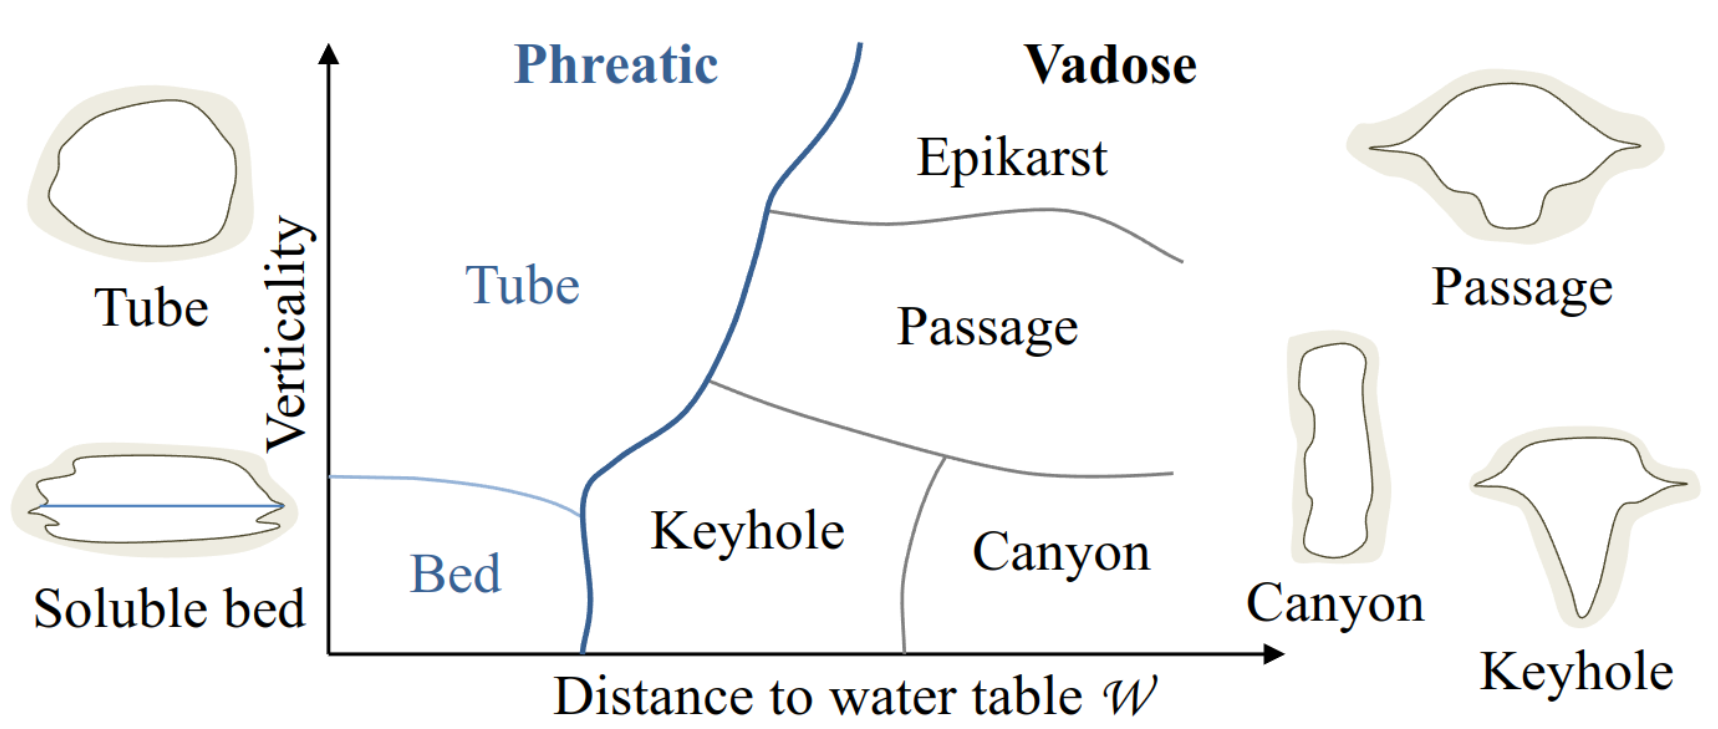
\includegraphics{KarstClassificationParis}
    \caption{Classification of tunnel shapes}
    \label{fig:karsts_tunnel-classif}
\end{figure}

\section{User control}
\label{sec:karsts_user-control}
- Importance of keeping user control \\
** Shape of a karst is close to randomness \\
** Want to be predictible \\
- Manipulation of control points \\
** Source \\
** Sink \\
- Paths tortuosity \\
- Inclusion of soil properties in the formation of paths, using the gradient of: \\
** Humidity, \\
** Porosity \\
- Real-time editing \\
** Allows for precise manipulation \\
- ...

\section{Results}
\label{sec:karsts_results}
- ... 

\section{Conclusion}
\label{sec:karsts_conclusion}
- ...